%\documentclass[aspectratio=43]{beamer}
\documentclass[t]{beamer}
\usetheme{ffmodern}  %% Themenwahl

\usepackage[ngerman]{babel} 
\usepackage[T1]{fontenc}    % richtige Silbentrennung
\usepackage[utf8]{inputenc} % Umlaute etc.!
\usepackage{eurosym}
\usepackage{tikz}
\usepackage{pgffor}

\usetikzlibrary{arrows,decorations.pathmorphing,backgrounds,fit,positioning,shapes.symbols,chains}

%-----------------
\title{Freifunk Hamburg}
%\author{In Hamburg funkt man frei\newline\newline\newline\newline\newline\newline\newline\newline Matthias Marx}
\author{Freies WLAN in den Häusern\newline\newline\newline\newline\newline\newline\newline\newline Matthias Marx}
\date{23. November 2018}
\license{CC-BY-3.0}

\begin{document}
  \maketitle
  
  %-----------------  
  \begin{frame}{Was ist Freifunk?}
    \begin{itemize}
      \item Initiative für freie, offene, kostenlose Netzwerke
      \item Steht allen offen, als Nutzer oder Anbieter
      \item Nichtkommerzielles Netz in Nutzerhand
      %\item Nutzt freie, quelloffene Programme
      %\item Netzneutral
    \end{itemize}
  \end{frame}
  
  %-----------------
  \begin{frame}{Verbreitung}
    \begin{columns}
      \begin{column}{0.6\textwidth}
  \begin{itemize}
    \item \href{http://freifunk.net/wie-mache-ich-mit/community-finden/}{443 Orte} mit 49.540 Zugangspunkten
    \item Zunehmend Unterstützung durch Bund und Länder
  \end{itemize}
      \end{column}
      \begin{column}{0.4\textwidth}
  \begin{center}
    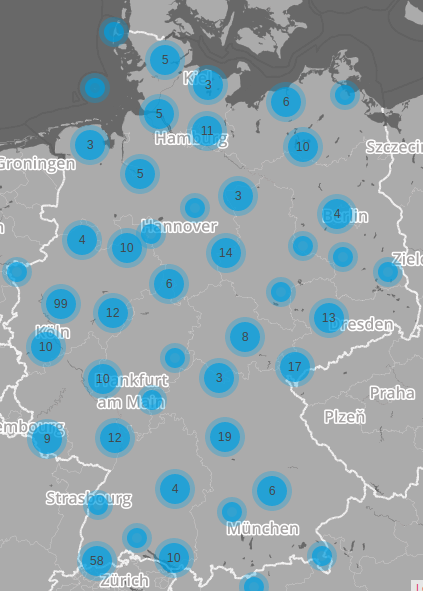
\includegraphics[width=\textwidth]{Bilder/community-map-2017-04-24}
  \end{center}
      \end{column}
    \end{columns}
  \end{frame}
  
  %----------------- 
  \begin{frame}{Freifunkknoten}
    \begin{center}
      \includegraphics[width=.6\textwidth]{Bilder/841}
    \end{center}
  \end{frame}
  
  %-----------------
  \begin{frame}{Knotenkarte}
    \begin{center}
      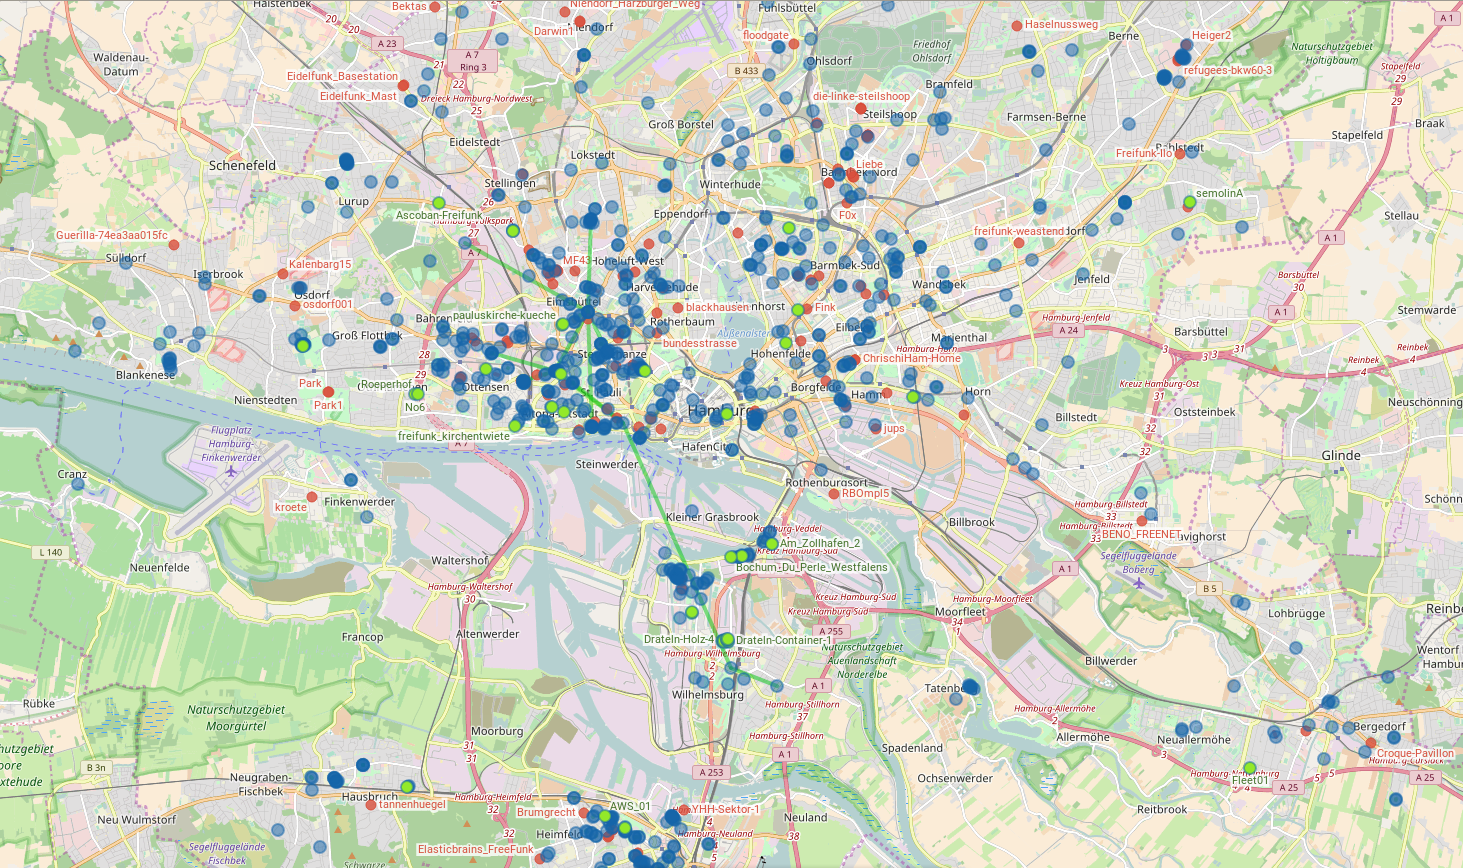
\includegraphics[width=.9\textwidth]{Bilder/knotenkarte-2017-04-24}
      \newline\tiny{Leaflet | © CC-BY-SA OpenStreetMap, andere}
    \end{center}
    Mehr als 950 Knoten in Hamburg, bis zu 3000 Geräte im Netz
  \end{frame}

  %----------------- 
  \foreach \index in {1, ..., 4} 
  {
    \begin{frame}{Das Netzwerk}
      \centering \includesvg[width=9cm]{netz-\index}
    \end{frame}
  }
  
  %-----------------
  \begin{frame}{Störerhaftung}
    \begin{itemize}
      \item Abgeschafft.
    \end{itemize}
  \end{frame}
  
%-----------------
  \begin{frame}{Störerhaftung}
    \begin{itemize}
      \item Keine Haftung für Knotenbetreiber
      \item Internetverkehr geht über unsere Gateways. Haftungsbefreiung nach TMG\S8.
      \item Wir nehmen die gesetzlichen Vorschriften wörtlich: Wir sammeln keine Daten.
    \end{itemize}
  \end{frame}  
  
  %-----------------
  \begin{frame}{\href{http://wiki.freifunk.net/Freifunk_Hamburg/Richtfunknetz}{Richtfunknetz}}
    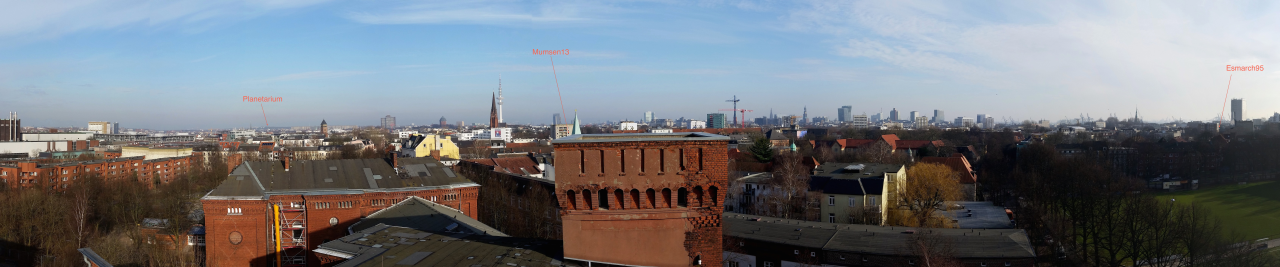
\includegraphics[width=\textwidth]{Bilder/fux}
    \begin{columns}
      \begin{column}{0.7\textwidth}
  \begin{itemize}
    \item Eigene Infrastruktur
    \begin{itemize}
      \item Redundanz und Lastverteilung 
      \item Unabhängig von Internetprovidern
    \end{itemize}
  \end{itemize}
      \end{column}
      \begin{column}{0.3\textwidth}
	\begin{center}
	  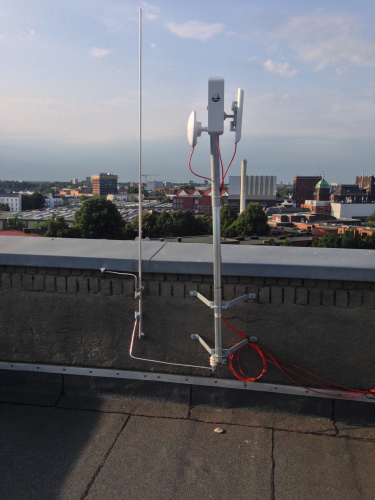
\includegraphics[width=.9\textwidth]{Bilder/richtfunkmast}
	\end{center}
      \end{column}
    \end{columns}
  \end{frame}
  
  %-----------------
  \begin{frame}{Richtfunknetz}
    \begin{center}
      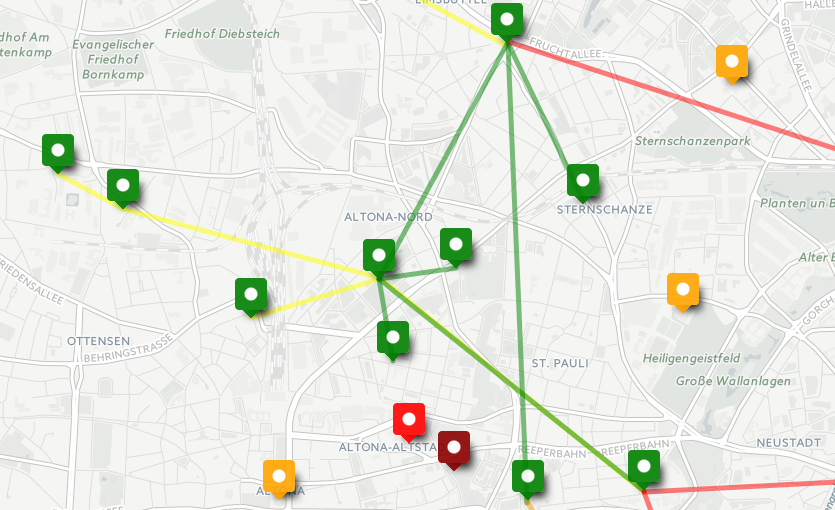
\includegraphics[width=0.95\textwidth]{Bilder/richtfunk-uebersicht}
    \end{center}
    \tiny{OSM - Deutschland Karte hergestellt aus OpenStreetMap-Daten | Lizenz: Open Database License (ODbL) | Courtesy of OpenStreetMap.de}
  \end{frame}
  
  %-----------------
  \begin{frame}{Freifunk für Geflüchtete}
    \begin{itemize}
      \item 2013: Embassy of Hope
      \item 2014: Schwarzenbergplatz
      \item 2015 \& 2016
      \begin{itemize}
       \item Flüchtlingsschiff Transit
       \item Messehallen
       \item Hauptbahnhof
       \item Baumärkte
       \item ZEA Schnackenburgallee (> 3000)
       \item Zahlreiche weitere Standorte
      \end{itemize}
    \end{itemize}
  \end{frame}
  
  
  %-----------------
  \begin{frame}{Aktuelles}
    \begin{itemize}
      \item Vorratsdatenspeicherung
      \item Störerhaftung
      \item Gemeinnützigkeit
    \end{itemize}
  \end{frame}
    
  
  %-----------------
  \begin{frame}{Howto?}
    \begin{itemize}
      \item Uplink finden
      \item Hardwarebedarf schätzen
      \item Geräte finanzieren und aufstellen
      \item Dokumentieren\\
      \small{ \href{https://wiki.freifunk.net/Hamburg}{wiki.freifunk.net/Hamburg}}
    \end{itemize}
  \end{frame}
  
  %-----------------
  \begin{frame}{Freifunk lebt vom Mitmachen}
    \begin{itemize}
      \item Wir sind kein Dienstleister
      \item aber wir geben unser Wissen gerne weiter
    \end{itemize}
  \end{frame}
  
  %-----------------
  \begin{frame}{Wie kann ich mitmachen?}
    \begin{itemize}
      \item Router aufstellen
      \item Freifunk-Treffen
      \begin{itemize}
       \item Montags, 19 Uhr, CCCHH, Zeiseweg 9
       \item Techniktreffen Freitags, 19:30 Uhr, Attraktor, Eschelsweg 4
      \end{itemize}
      \item Webseite\\
      \href{https://hamburg.freifunk.net}{\small hamburg.freifunk.net}
      \item Mailingliste\\
      \href{mailto:freifunk@hamburg.ccc.de}{\small freifunk@hamburg.ccc.de}
      \item IRC\\
      \small{\#ffhh auf irc.hackint.org}
    \end{itemize}
  \end{frame}
  
  %-----------------
  \begin{frame}{Vielen Dank!}
    \begin{columns}
      \begin{column}{0.5\textwidth}
        \centering
        \includesvg[width=3.5cm]{in-hamburg-funkt-man-frei}
      \end{column}
      
      \begin{column}{0.5\textwidth}
        \centering
        
\includegraphics[width=0.65\textwidth]{Bilder/qrcode-2018-11-23}
      \end{column}
    \end{columns}   
    
    \begin{itemize}
      \item \textbf{WWW} \href{https://hamburg.freifunk.net}{hamburg.freifunk.net}
      \item \textbf{Mail} \href{mailto:kontakt@hamburg.freifunk.net}{kontakt@hamburg.freifunk.net}
      \item \textbf{Treffen} Montags \& Freitags\\\href{https://hamburg.freifunk.net/kalender}{\small hamburg.freifunk.net/kalender}
    \end{itemize}
  \end{frame}
  
\end{document}
